\section{Struttura dei dispositivi di memorizzazione}
    I \textbf{dischi magnetici} e i \textbf{dispositivi NVM} (\textit{non volatile memory}) costituiscono i principali supporti di memoria secondaria nei moderni computer. Andiamo a descriverne la struttura e in che modo i sistemi operativi riescano a tradurre le loro proprietà fisiche in memoria logica tramite la mappatura degli indirizzi.
    
    \subsection{Dischi rigidi}
        Concettualmente, la struttura di un disco rigido è abbastanza semplice: sono simili a dei cd divisi in \textit{settori}, a loro volta organizzati \textit{tracce}. Se prendiamo tutte le tracce corrispondenti verticalmente, una per ogni disco, abbiamo un \textit{cilindro}.
        
        Le dimensioni del settore sono state per molto tempo di 512 byte, ma dal 2010 i produttori hanno iniziato a migrare verso una soluzione di 4KB per settore.
        
        \begin{figure}[h]
            \centering
            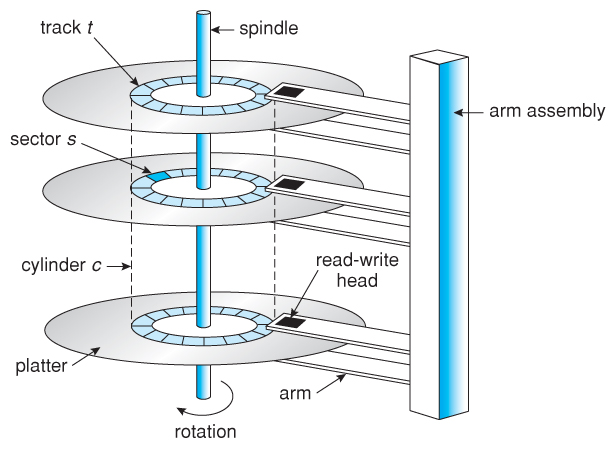
\includegraphics[width = 0.8\textwidth]{img/hd.jpg}
            \caption{Struttura di un disco rigido}
            \label{fig:my_label}
        \end{figure}
        
        \paragraph{Aspetto meccanico.} Quando un disco è in funzione, un motore lo fa ruotare ad alta velocità, la quale è spesso espressa in termini di RPM, ossia giri al minuto, i quali possono variare da 5400 a 15000. Un altro aspetto relativo alle prestazioni è il \textbf{tempo di posizionamento}, composto dal tempo necessario a spostare il braccio del disco in corrispondenza del cilindro desiderato, e il tempo necessario affinché il settore desiderato si posti, tramite la rotazione, sotto la testina.
        
        Il fenomeno dell'\textbf{urto della testina} avviene quando la testina danneggia il disco magnetico, e comporta la sostituzione dell'intera unità di memoria e la perdita dei dati.
        
    \subsection{Dispositivi NVM}
        I dispositivi NVM sono elettrici anziché meccanici, e questo permette delle performance e una durabilità maggiori rispetto a quelli classici. Una grande parte di essi sono costituiti da un controllore e da diversi chip di memoria a semiconduttore NAND flash. Esistono altre tecnologie ma sono molto meno popolari.
        
        Questi dispositivi sono spesso inseriti in contenitori simili a unità disco, e per questo motivo vengono spesso chiamati \textbf{dischi a stato solido}, o \textbf{SDD} (\textit{solid state drive}). In altri casi può assumere altre forme, come le chiavette USB o un chip installato direttamente sulla scheda madre, come sugli smartphone. In ogni caso, possiamo discutere di questi dispositivi alla stessa maniera, in quanto si comportano allo stesso modo.
        
        Come abbiamo detto, questi dispositivi sono \textbf{più efficienti} delle controparti classiche in quanto non hanno bisogno di posizionamento meccanico, più resistenti ai guasti per lo stesso motivo e consumano meno energia. D'altro canto sono più costosi e tendono ad avere una capacità minore. Questi fattori sono tuttavia in costante miglioramento col passare degli anni.
        
        In funzione dell'alta velocità di trasferimento di questi dispositivi, l'interfaccia bus può costituire un \textbf{bottleneck} non indifferente al throughput, e quindi alcuni dispositivi NVM si connettono direttamente al bus di sistema.
        
        Le caratteristiche dei semiconduttori NAND portano tuttavia \textbf{nuove sfide}: nonostante sia possibile eseguire scritture a livello di pagina, non è possibile sovrascrivere dati, e quindi occorre eseguire una cancellazione (operazione molto costosa, anche perché si verifica a livello di blocchi di diverse pagine) prima di riscrivere. In una certa misura ciò è limitato da un certo livello di parallelismo offerto da questi dispositivi, grazie ai molti \textbf{datapath} di cui dispongono.
        
        Inoltre l'\textbf{usura} dei dispositivi NVM dipende dall'utilizzo: in media un semiconduttore NAND si deteriora e diventa inutilizzabile dopo 100.000 cicli, e la durata di un tale dispositivo non viene espressa in anni ma in base al numero di scritture al giorno.
        
        Queste limitazioni hanno portato allo sviluppo di algoritmi di miglioramento che fortunatamente non sono a carico del sistema operativo ma del dispositivo, rendendolo dunque più intelligente.
        
\section{Gestione delle unità di memoria secondaria}
    Il sistema operativo è responsabile di alcuni aspetti della gestione delle unità di memoria a disco: discutiamo in questo paragrafo l'inizializzazione del dispositivo, l'avviamento del sistema dal dispositivo e la gestione di blocchi difettosi.
    
    \subsection{Formattazione del disco, partizioni e volumi}
        Un dispositivo di memorizzazione nuovo non contiene nulla, ma deve essere inizializzato e diviso in settori che possano essere scritti o letti dal controllore, processo chiamato \textbf{formattazione di basso livello} o \textbf{formattazione fisica}. Essa riempie il dispositivo con una speciale struttura dati per ogni locazione di memorizzazione, la quale consiste tipicamente di un'intestazione, un'area per i dati e una coda. La prima e l'ultima contengono informazioni usate dal controllore del disco come per esempio il numero del settore e un codice per la correzione di errori.
        
        La formattazione fisica è spesso parte del processo di produzione dell'hardware, in maniera che il produttore possa testare il disco. Una delle scelte fatte in questa fase è la dimensione dei settori, spesso ristretta a poche opzioni come 512 byte e 4 Kb. La maggiore dimensione di settori implica la presenza di meno settori per ogni striscia, ma anche una minor quantità di code e intestazioni, e quindi in definitiva più spazio di archiviazione.
        
        Prima di usare il disco come contenitore per i file, il sistema operativo deve prima registrare le sue strutture dati sullo stesso, cosa che fa in tre passi:
        \begin{itemize}
            \item Suddividere il disco in uno o più blocchi di blocchi, dette \textbf{partizioni}. Il sistema può trattare ogni partizione come se fosse un dispositivo a sé, e infatti spesso ciò avviene nella misura in cui viene installato un intero sistema operativo su ogni partizione.
            
            \item Creazione e gestione del volume. A volte ciò è implicito, come quando un file system viene inserito direttamente in una partizione la quale è poi pronta a essere montata e usata, altre volte è esplicito.
            
            \item La \textbf{formattazione logica}, ossia la creazione del file system; il sistema operativo registra nel dispositivo le strutture dati iniziali relative al file system, le quali possono includere descrizioni dello spazio libero, dello spazio occupato e una cartella iniziale vuota.
        \end{itemize}
        
        Alcuni sistemi operativi permettono a certi programmi di impiegare una partizione del disco come un grande array sequenziale di blocchi logici, non contenente alcuna struttura dati relativa al file system. Questo array è detto \textbf{disco di basso livello} (\textit{raw disk}). Il relativo I/O si chiama \textbf{I/O di basso livello}. Una tale struttura può per esempio essere usata come spazio di swap. Nonostante alcuni programmi potrebbero essere più efficienti tramite un tale tipo di accesso, la maggior parte preferiscono usare il file system fornito anziché farsi carico della gestione dei dati.
        
    \subsection{Blocco d'avviamento}
        Affinché un computer possa entrare in funzione, all'avvio o riavvio, è necessario che esegua un programma iniziale. Di solito questo \textit{bootstrap} è piuttosto semplice. Esso è spesso memorizzato nel \textit{firmware} ed è posizionato su una memoria NVM sulla scheda madre, e mappato su una locazione di memoria nota.
        
        Il piccolo programma di avviamento del bootstrap, il \textit{bootstrap loader}, è capace di caricare il bootstrap completo, il quale a sua volta è più complesso e può caricare tutto il sistema operativo e inizializzare ogni aspetto del computer.
        
    \subsection{Blocchi difettosi}
        Le unità a disco sono strutturalmente soggette a guasti, a causa delle varie parti meccaniche mobili. Alcuni di questi possono portare a errori irreparabili, e causare quindi il cambio dell'intera unità, ma possiamo anche trovare \textbf{blocchi difettosi} (\textit{bad blocks}). Ciò è così comune che la maggior parte delle unità messe in commercio già contengono blocchi difettosi.
        
        Se si trovano blocchi difettosi durante la formattazione, essi possono essere marcati come non utilizzabili. Se un blocco diviene difettoso durante l'uso del disco, deve essere lanciato un programma specifico che li individua. Spesso il suo contenuto viene perso.
        
        Unità a disco più complesse hanno strategie più raffinate per trattare i blocchi difettosi: li individua e li lista già in fase di produzione, e questa lista viene tenuta aggiornata per tutta la durata operativa dell'unità. Inoltre viene tenuta una lista di blocchi nascosti che possono essere sostituiti logicamente a quelli difettosi. Quest'ultima strategia è nota come \textbf{accantonamento dei settori} (\textit{sector sparing} o \textit{forwarding}).
        
        Questo potrebbe inficiare sulle prestazioni, e infatti molti dischi tengono blocchi di riserva per ogni cilindro, in maniera tale da non dover riposizionare la testina.
        
        Un'alternativa è la \textbf{traslazione dei settori}, o \textit{sector slipping}: se il blocco 10 è malfunzionante e il primo blocco di riserva libero è il 140, tutti i settori dal 10 al 139 vengono spostati in avanti di una posizione.
        
        In generale, un errore è \textit{reversibile} quando possiamo in qualche modo recuperare il contenuto del blocco, mentre è \textit{irreversibile} quando ciò non si può fare e dobbiamo quindi ricorrere a un backup, operazione da eseguire manualmente.
        
        Anche i dispositivi NVM possono avere pagine difettose, ma in questo caso la soluzione non incide sul tempo di riposizionamento, e quindi gli algoritmi sono più semplici ed efficienti.
        
\section{Gestione dell'area di avvicendamento (swap space)}
    Abbiamo già parlato dello swapping: nel momento in cui ci siano troppi processi e la memoria si riempia, le prestazioni degradano e diventa necessario fare lo \textit{swap in} di processi per permettere a nuovi processi di entrare in memoria; nella pratica ciò è molto raro, in quanto fare lo \textit{swap out} di interi processi è inutile e dispendioso. Si manda in area di avvicendamento piuttosto una parte di un processo espressa in pagine, combinando quindi questo concetto con tecniche di memoria virtuale.
    
    La \textbf{gestione dell'area di swap} è un altro compito di basso livello del sistema operativo. Siccome come area di swap viene spesso usata un'unità a disco, il suo uso riduce notevolmente le prestazioni. Lo scopo è quindi realizzare un'area di swap che fornisca il miglior throughput possibile.
    
    \subsection{Uso dell'area di swap}
        L'uso di quest'area dipende dal sistema operativo: alcuni possono memorizzarvi le immagini di interi processi, altri solo delle pagine. Ne deriva che lo spazio richiesto da quest'area è molto variabile, dai megabyte ai gigabyte.
        
        Si noti che una stima per eccesso è meno dannosa di una per difetto, in quanto un'area di avvicendamento troppo grande spreca memoria altrimenti utilizzabile per i file, mentre una troppo piccola potrebbe richiedere la soppressione forzata di processi nel caso di esaurimento.
        
    \subsection{Collocazione dell'area di swap}
        Questa area può essere collocata all'interno del normale file system o in una partizione dedicata. Nel primo caso possiamo usare le ordinarie operazione per cercarla, darle un nome, etc, come gli altri file nel file system.
        
        In caso contrario abbiamo una \textit{raw partition} senza alcun file system, ma a cui  è più facile e veloce accedere. Questo causa una maggiore frammentazione, della quale tuttavia non ci preoccupiamo molto in quanto i file sulla partizione di swap hanno vita breve. Difatti questi vengono eliminati al riavvio del PC.
        
\section{Connessione dei dispositivi di memorizzazione}
    I calcolatori accedono alla memoria secondaria in tre modi: tramite un dispositivo collegato alla macchina, alla rete o tramite un dispositivo cloud.
    
    \subsection{Memoria secondaria connessa alla macchina}
        Alla memoria connessa alla macchina si accede dalle porte di I/O locale, le quali utilizzano diverse tecnologie, la più popolare delle quali è SATA.
        
        In architetture di fascia alta e server ci si può avvalere di diverse tecnologie come cavi di rame e fibra ottica.
        
        Anche i dispositivi sono omogenei, come per esempio unità a disco, Blu-Ray, dispositivi NVM.
        
    \subsection{Memoria secondaria connessa alla rete}
        Un \textbf{dispositivo NAS} (\textbf{network-attached storage}) fornisce accesso a spazio di archiviazione tramite la rete. Può essere costituito da un dispositivo specializzato o da un semplice computer che fornisce il suo spazio di memoria ad altri computer connessi attraverso la rete.
        
    \subsection{Memoria secondaria su cloud}
        Alcuni fornitori di servizi cloud forniscono spazio di archiviazione remoto, che prende il nome di \textit{cloud storage} ed è accessibile tramite Internet o altre reti WAN. Al contrario dei dispositivi NAS, il cloud storage presenta modalità di accesso basate su API, questo per far fronte alla maggiore latenza rispetto a una rete LAN e alla maggiore possibilità di perdita della connessione.
    
    \subsection{Storage-area network e storage array}
        Un problema dei sistemi di memoria connessi alla rete è che competono con gli altri servizi per la banda, dovendone occupare una quantità considerevole per le operazioni di I/O.
        
        Una \textbf{storage-area network (SAN)} è una rete privata che impiega protocolli specifici tra i server e le unità di memoria secondaria. Essa è molto flessibile e può per esempio connettersi a molte macchine, assegnare più memoria a quali ne abbiano bisogno, eccetera.
        
        Uno \textbf{storage array} è un dispositivo che può includere porte SAN, di rete o entrambe. Contiene unità per memorizzare dati, un controllore e permette l'accesso tramite la rete. I controllori sono composti da CPU, memoria e software e regolano le funzionalità dell'array, compresi protocolli, snapshot, duplicazione, crittografia, etc.
        
\section{Strutture RAID}
    Con il diminuire del costo delle unità di memorizzazione, possiamo avere più dischi nello stesso sistema, potenzialmente capaci di operare in parallelo. Questo presenta l'opportunità di memorizzare i dati in maniera ridondante, per diminuire la sensibilità ai fault. Ci sono vari metodi di organizzazione di queste strutture, noti come \textbf{batterie ridondanti di dischi} (\textit{redundant array of indipendent disks}, \textbf{RAID}).
    
    Storicamente una struttura RAID veniva impiegata per motivi economici (infatti la \textit{I} stava per \textit{inexpensive}), mentre oggi il motivo principale è l'affidabilità.
    
    \subsection{Miglioramento dell'affidabilità tramite la ridondanza}
        In una batteria di dischi, la possibilità di guasto di un qualsiasi disco è certamente più alta della probabilità di guasto di un disco preso singolarmente. Per questo viene introdotta una certa \textbf{ridondanza}, ossia la memorizzazione di informazioni non necessarie ma che in caso di guasto possono essere utili a ricostruire i dati persi. La stessa tecnica si può attuare per dispositivi NVM, ma non avendo parti meccaniche, questi ultimi sono meno soggetti ai guasti.
        
        Il metodo più semplice ma più costoso di ridondanza è il \textbf{mirroring}: ogni scrittura effettuata su un disco viene effettuata anche su un secondo disco identico. Perdiamo i dati solo nel caso si guasti un primo disco e prima della sostituzione si guasti anche il secondo, evento generalmente molto improbabile.
        
        Un problema particolarmente sentito è il calo di alimentazione elettrica: in questo caso i due dischi gemelli possono essere lasciati in uno stato incoerente se stavano scrivendo lo stesso dato sullo stesso blocco. Una possibile soluzione è scrivere prima su un disco e in secondo momento sul secondo disco. Un'altra soluzione è l'impiego di una \textbf{NVRAM}, \textit{non volatile RAM}, la quale è protetta dalla perdita di dati anche in caso di mancanza di corrente elettrica.
        
    \subsection{Miglioramento delle prestazioni tramite il parallelismo}
        Avere più dispositivi di memorizzazione in parallelo può migliorare drasticamente le prestazioni, distribuendo la lettura su più dispositivi: la forma più semplice di ciò è lo \textbf{striping}, e in particolare il \textit{bit-wise striping}. Ciò consiste nello scrivere i vari bit su dispositivi diversi. Per esempio se abbiamo otto dispositivi, possiamo scrivere un bit di ogni byte per ogni dispositivo. Quando andremo quindi a leggerli avremo la stessa velocità di accesso ma riusciremo a leggere otto volte più dati. Questo si può generalizzare per un numero di dispositivi che si divide per 8 o multiplo di 8.
        
        Chiaramente lo striping non deve necessariamente avvenire a livello di bit, e infatti la versione più popolare è a livello di blocco.
        
    \subsection{Livelli RAID}
        La tecnica di \textbf{mirroring} offre una grande affidabilità ma nessun miglioramento alle prestazioni, mentre quella di striping l'esatto opposto. Sono state proposti diversi schemi per unire le due cose, e in particolare i compromessi fra costi e prestazioni sono stati classificati in livelli chiamati \textbf{RAID}. Vengono usati 4 dischi per la memorizzazione standard, e gli altri sono dedicati a fornire ridondanza allo scopo di assicurare una maggiore sicurezza.
        
        \begin{itemize}
            \item \textbf{RAID di livello 0.} Questo livello si riferisce a dischi con striping a livello di blocchi ma senza ridondanza.
            
            \item \textbf{RAID di livello 1.} Questo livello si riferisce alla tecnica di mirroring.
            
            \item \textbf{RAID di livello 4.} Anche noto come \textbf{organizzazione con codici per la correzione di errori di memoria (ECC)}. Tale organizzazione è anche usata nei RAID di livello 5 e 6.
            
            Possiamo usare gli \textbf{ECC} (\textit{error-correcting codes}) negli array di memorizzazione facendo lo striping di $n$ bit su $n$ dispositivi per esempio, e usando ulteriori dispositivi $P$ per memorizzare i bit di correzione, con un'idea molto semplice: se un settore è danneggiato sappiamo precisamente di quale settore si tratta, e possiamo andare a calcolare la parità dei bit negli altri settori e compararla con l'ECC in $P$. Se la parità corrisponde il bit danneggiato è 0, altrimenti è 1.
            
            Questo livello di RAID presenta la stessa protezione dei dati del livello 1, ma guadagna in termini di parallelismo a causa dello striping, e inoltre usa un solo disco per la correzione degli errori, anziché multipli dischi di mirroring.
            
            Un problema di prestazioni del RAID di livello 4, come di tutti i livelli basati su \textbf{bit di parità}, sta nella scrittura e nell'aggiornamento di questo bit. Questo problema è tuttavia diminuito nei sistemi moderni che sono più performanti e che talvolta delegano questo compito ai controllori dei dispositivi di memorizzazione, oltre che avere delle cache per memorizzare blocchi mentre viene calcolata la parità, rendendo questo metodo talvolta anche più veloce di un'organizzazione senza cache e senza parità.
            
            \item \textbf{RAID di livello 5.} Il livello 5, o \textbf{organizzazione con blocchi intercalati a parità distribuita}, differisce dal livello precedente in quanto anziché memorizzare nei primi $n$ dischi i dati e nell'$n+1$ le informazioni di parità, entrambe sono distribuite nelle $n+1$ unità. Per ogni blocco, una delle unità memorizza la parità e le altre i dati, con la restrizione che una unità che contiene le informazioni di parità di un certo blocco non ne può contenere anche i dati, in quanto il guasto di questa unità provocherebbe la perdita sia dei dati che delle informazioni di parità.
            
            Questa organizzazione permette un utilizzo meno intensivo delle unità, in quanto nella precedente quella che memorizzava le informazioni di parità era molto utilizzata. RAID 5 è l'organizzazione più comune.
            
            \item \textbf{RAID di livello 6.} Detto anche \textbf{schema di ridondanza P+Q}, è molto simile al livello 5 ma utilizza più informazioni ridondanti per far fronte a guasti simultanei di dischi. La parità XOR non può essere usata perché essendo i due bit di parità uguali non darebbe informazioni utili. Per calcolare Q vengono invece usati codici di errore basati sulla \textbf{matematica dei campi di Galois}.
            
            \item \textbf{RAID di livello 6 multidimensionale.} Alcuni sofisticati storage array ampliano il livello 6. Immaginiamo di avere molte unità di memorizzazione; distribuirle in fila con solo due unità di correzione (P e Q) per tutte loro sarebbe riduttivo. Vengono dunque distribuite in righe e colonne (array di dimensione 2 o superiore) e per ogni riga e ogni colonna vengono dedicate due unità di correzione, in modo da poter correggere uno o più errori. Le unità di correzione sono distribuite, come abbiamo visto in precedenza.
            
            \item \textbf{RAID di livello 0 + 1 e 1 + 0.} Il livello 0 + 1 consiste in una combinazione dei livelli 0 e 1, dove il livello 0 fornisce le prestazioni mentre l'1 l'affidabilità. Si effettua lo striping su un insieme di dischi e si duplica ogni sezione tramite la tecnica del mirroring.
            
            Il RAID di livello 1 + 0 prevede di fare il mirroring delle unità a coppie e poi lo striping di queste coppie.
        \end{itemize}
        
        Sono state proposte molte varianti ai livelli di base sopra citati, e un altra variante da considerare è l'implementazione. Ecco alcuni degli strati architetturali a cui è possibile implementare un sistema RAID.
        \begin{itemize}
            \item A livello software tramite il programma per la gestione dei volumi. In questo caso possiamo ottenere un sistema RAID completo anche se i dispositivi di memorizzazione non offrono moltissime funzionalità adatte allo scopo.
            
            \item A livello hardware dall'adattatore del bus della macchina. Solo i dischi connessi a questo bus possono costituire parte integrante dell'array RAID. Soluzione a basso costo ma poco flessibile.
            
            \item A livello hardware dall'array di dischi. Soluzione molto più flessibile della precedente.
            
            \item Implementato da dispositivi di virtualizzazione del disco a livello di interconnessione SAN. In questo caso il dispositivo di memorizzazione funge da intermediario tra le macchine e l'area di memorizzazione, accettando istruzioni dai server e gestendo l'accesso alla memoria secondaria. Potrebbe, per esempio, effettuare il mirroring.
        \end{itemize}
        
        Altre funzionalità, come quella di \textit{snapshot} e di \textbf{replica}, possono essere implementate per ognuno di questi livelli.
        
        Uno snapshot è un'immagine del file system così com'era prima dell'ultimo aggiornamento. La replica, che può essere sincrona o asincrona, prevede il caricamento dei dati su diversi siti, per prevenire perdita dei dati o per finalità di ridondanza.
        
        Un'altra caratteristica dei sistemi RAID è la presenza di \textbf{dischi di scorta}, che permettono a guasti di essere prontamente riparati senza dover attendere la sostituzione del disco.